\documentclass[tikz,border=6pt]{standalone}
\usepackage{helvet}
\renewcommand{\familydefault}{\sfdefault}
\begin{document}
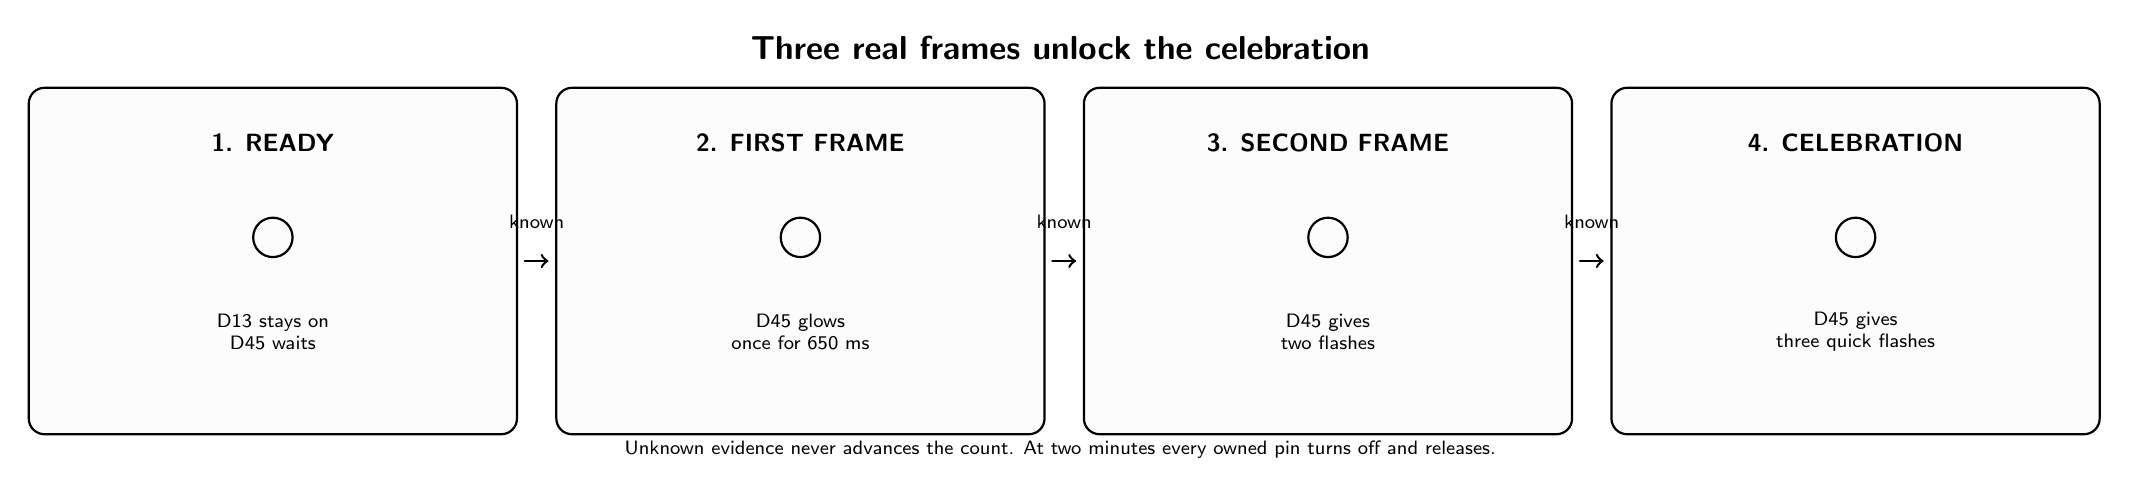
\begin{tikzpicture}[x=1mm,y=1mm,line cap=round,line join=round,
  box/.style={draw,line width=.8pt,rounded corners=2mm,minimum width=62mm,
              minimum height=44mm,align=center,fill=black!1},
  lamp/.style={circle,draw,line width=.8pt,minimum size=5mm},
  small/.style={font=\scriptsize}]
\node[font=\bfseries\large] at (134,56)
  {Three real frames unlock the celebration};
\foreach \x/\title in
  {34/1. READY,
   101/2. FIRST FRAME,
   168/3. SECOND FRAME,
   235/4. CELEBRATION}
{
  \node[box] at (\x,29) {};
  \node[font=\bfseries\small] at (\x,44) {\title};
  \node[lamp] at (\x,32) {};
}
\node[small,align=center] at (34,20) {D13 stays on\\D45 waits};
\node[small,align=center] at (101,20) {D45 glows\\once for 650 ms};
\node[small,align=center] at (168,20) {D45 gives\\two flashes};
\node[small,align=center] at (235,20) {D45 gives\\three quick flashes};
\draw[->,line width=.9pt] (66,29)--(69,29);
\draw[->,line width=.9pt] (133,29)--(136,29);
\draw[->,line width=.9pt] (200,29)--(203,29);
\node[small] at (67.5,34) {known};
\node[small] at (134.5,34) {known};
\node[small] at (201.5,34) {known};
\node[small,align=center] at (134,5)
  {Unknown evidence never advances the count. At two minutes every owned pin turns off and releases.};
\end{tikzpicture}
\end{document}
